\documentclass[12pt]{article}

\setlength\parindent{0pt}

\usepackage[norsk]{babel}
\usepackage{graphicx}
\usepackage{amsmath}
\usepackage{tikz}
\usepackage{hyperref}
\usepackage{graphicx}
\usepackage[a4paper, total={6.25in, 9.5in}]{geometry}
\setlength{\voffset}{0.25in}
\setlength{\headsep}{5pt}
\setlength{\parskip}{1em}
\usepackage{listings}

\definecolor{pblue}{rgb}{0.2,0.2,0.7}
% \definecolor{pgreen}{rgb}{0,0.5,0}
\definecolor{pred}{rgb}{0.7,0.2,0.2}
\definecolor{pgrey}{rgb}{0.46,0.45,0.48}


\hbadness=10000

\usetikzlibrary{automata, positioning, arrows}

\tikzset{
	->,
	node distance=3cm,
	initial text=$ $,
}

\title{Code clones thesis proposal}




\begin{document}
\maketitle

\section*{Motivation}
\begin{itemize}
	\item  Modern clone detection tools are as far as I've seen not very suitable for use while
	      programming, but rather for analysis after code has been written. It seems
          likely that managing these clones when analyzed later is harder than managing
          code clones detected in real-time.
	\item One plugin for Eclipse exists already, but the plugin does not have
        functionality for merging clones.
    \item No tools I've seen provide ``real-time`` clone detection and functionality to merge
	      them.

\end{itemize}

\section*{Proposal}
I want to develop a tool which provides real-time clone detection and functionality to
merge the detected clones in a modern IDE. This could be suitable to implement as an LSP
server, making it an IDE agnostic tool.
\subsection*{Potential research questions}

\begin{itemize}
	\item How could real-time detection of code clones affect code quality compared to
	      later analysis?

	\item How should real-time code clone detection be implemented when focusing on efficiency and
	      scalability?

	\item How should real-time code clone merging be implemented when focusing on efficiency and
	      scalability?

	\item How should code clone detection be offered to IDE users? (LSP, plugins, ...)
\end{itemize}

\subsection*{Things to research and challenges}
\begin{itemize}
    \item Real-time clone detection (while typing in an IDE)
    \item Refactoring-Oriented clones
    \item Code clone merging
    \item Incremental code clone detection?
    \item Efficient detection of new code clones in a changing codebase
    \item Providing clone detection as an LSP server or plugin
\end{itemize}

\subsection*{Previous work / competition}
\begin{itemize}
    \item SimEclipse: An Eclipse plugin. \url{https://clones.usask.ca/pubfiles/articles/UddinIntegratedCM_CSACON-2015.pdf}
\end{itemize}

\subsection*{Tools of relevance}
\begin{itemize}
    \item SimLib: a clone detection engine/library written in Java 
        \url{https://github.com/suddin/ca.usask.cs.srlab.simLib}
    \item lsp4j: A Java library for creating LSP servers \url{https://github.com/eclipse/lsp4j}
\end{itemize}

\subsection*{Current title in mind}
\begin{itemize}
    \item ``Towards modern support for clone management in IDE's``
    \item ``Real-time management of code clones in an IDE environment``
\end{itemize}

\subsection*{Going Forward}

Going forward I will for the rest of the semester focus on:

\begin{itemize}
    \item Getting an overview of existing techniques for both detection and merging of
        clones
    \item Determine if LSP is an appropriate protocol for implementing this tool
    \item Read more about general refactoring and software quality for the essay
\end{itemize}

\subsection*{Relevant points from articles I've read}

\begin{center}

    From \url{https://link.springer.com/chapter/10.1007/978-981-16-1927-4_4}
    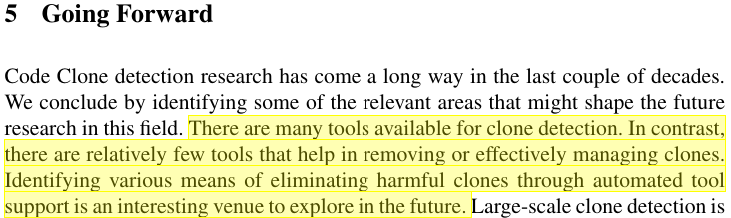
\includegraphics[width=450px]{images/sourcerercc.png}
    \noindent\rule{8cm}{0.4pt}

    From \url{https://www.researchgate.net/publication/353661146_NiCad_A_Modern_Clone_Detector}
    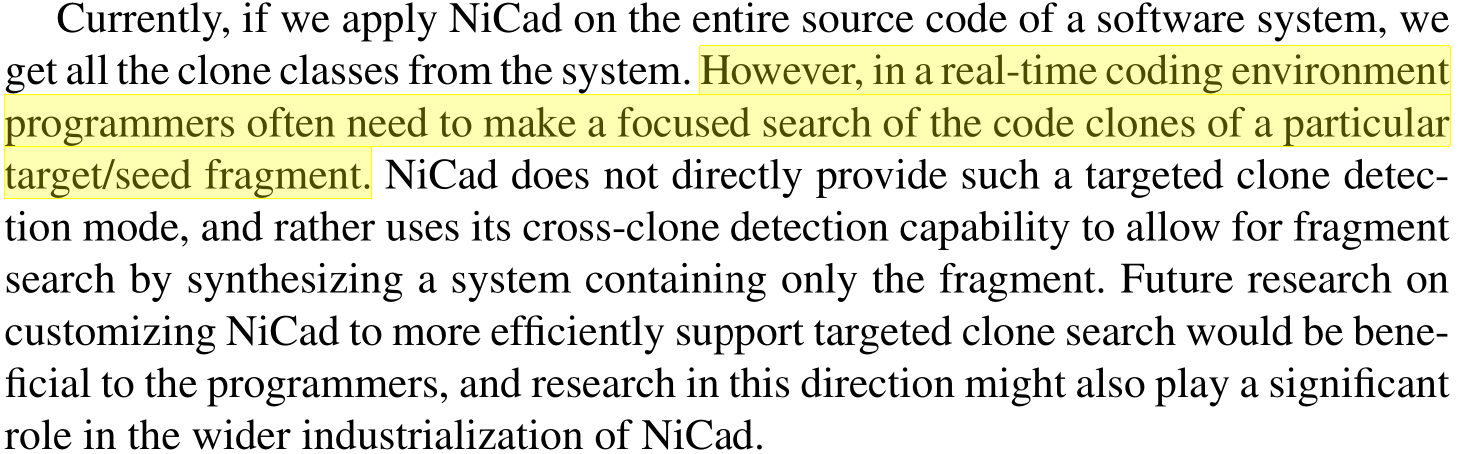
\includegraphics[width=450px]{images/nicadquote.png}
    \noindent\rule{8cm}{0.4pt}

    From \url{https://link.springer.com/chapter/10.1007/978-981-16-1927-4_13}
    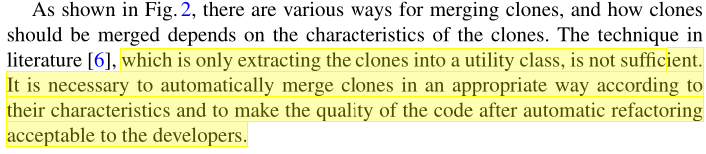
\includegraphics[width=450px]{images/refactoringoriented.png}
    \noindent\rule{8cm}{0.4pt}

    From \url{https://www.sciencedirect.com/science/article/pii/S1877050918308123}
    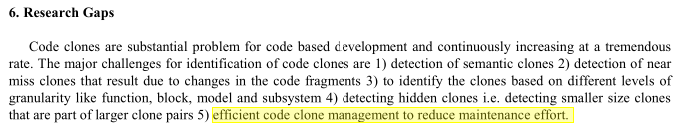
\includegraphics[width=450px]{images/managementquote.png}
\end{center}

\end{document}
